%%%%%%%%%%%%%%%%%%%%%%%%%%%%%%%%%%%%%%%%%%%%%%%%%%%%%%%%%%%%%%%%%%%%%%%%%%%%%%%%%%%%%
%                        Author: Harshit Prashant Dhanwalkar                        %
%%%%%%%%%%%%%%%%%%%%%%%%%%%%%%%%%%%%%%%%%%%%%%%%%%%%%%%%%%%%%%%%%%%%%%%%%%%%%%%%%%%%%

%-------------------------------------------------------------------------------------
%                    PACKAGES AND OTHER DOCUMENT CONFIGURATIONS                      %
%-------------------------------------------------------------------------------------
\documentclass[fleqn,10pt]{SelfArx} % Document font size and equations flushed left
\usepackage[english]{babel} 
\usepackage{enumitem}

\usepackage{tikz}
\usetikzlibrary{trees, positioning, shapes}
\usepackage{tikz-3dplot}
\tikzstyle{vertex}=[draw,fill=black!15,circle,minimum size=20pt,inner sep=0pt]
\tikzstyle{selected edge} = [draw,line width=5pt,-,red!50]

\usepackage{amsmath}
\usepackage{array} % for tables

\usepackage{mathtools}

\usepackage{pgfplots}
\pgfplotsset{compat=1.18}
\tdplotsetmaincoords{60}{115}
\pgfplotsset{compat=newest}

%-------------------------------------------------------------------------------------
%                                       COLUMNS                                      %
%-------------------------------------------------------------------------------------
\setlength{\columnsep}{0.55cm} % Distance between the two columns of text
\setlength{\fboxrule}{0.75pt} % Width of the border around the abstract

%-------------------------------------------------------------------------------------
%                                        COLORS                                      %
%-------------------------------------------------------------------------------------
\definecolor{color1}{RGB}{0,0,90} % Color of the article title and sections
\definecolor{color2}{RGB}{0,20,20} % Color of the boxes behind the abstract and headings

%-------------------------------------------------------------------------------------
%                                       EQUATIONS                                    %
%-------------------------------------------------------------------------------------
\usepackage{cancel} % for crossing the word showing it is cancelled or is zero

%-------------------------------------------------------------------------------------
%                                     EQUATIONLINKS                                  %
%-------------------------------------------------------------------------------------
\newcommand{\myeqref}[1]{Eq.\textcolor{blue}{\textup{(\getrefnumber{#1})}}}

%-------------------------------------------------------------------------------------
%                                       HYPERLINKS                                   %
%-------------------------------------------------------------------------------------
\usepackage{xcolor}
\usepackage{hyperref}
\usepackage{footnote}

%\newcommand{\myhref}[2]{\href{#1}{\textcolor{blue}{#2}}}
\newcommand{\myhref}[2]{%
  \href{#1}{\textcolor{blue}{#2}}%
  \footnote{\url{#1}}%
}

\usepackage{cleveref}
% Customize cleveref to use "Eq." for equations
\crefname{equation}{Eq.}{Eq.}
\Crefname{equation}{Eq.}{Eq.}

\hypersetup{
	hidelinks,
	colorlinks,
	breaklinks=true,
	urlcolor=color2,
	citecolor=color1,
	linkcolor=color1,
	bookmarksopen=false,
	pdftitle={Title},
	pdfauthor={Author},
}

% ------------------------------------------------------------------------------------
%                                       CUSTOM  SYMBOLS                              %
%-------------------------------------------------------------------------------------
\newcommand{\zbar}{\raisebox{0.2ex}{--}\kern-0.6em Z}

% ------------------------------------------------------------------------------------
%                                       CUSTOM  YELLOW STICKY NOTES		     %
%-------------------------------------------------------------------------------------
\usepackage{color}
\usepackage{calc}

\setlength{\parskip}{0ex}
\setlength{\parindent}{0ex}

\newlength{\yellownotewidth}
\setlength{\yellownotewidth}{2.5cm}
\newlength{\yellownoteheight}
\setlength{\yellownoteheight}{2.5cm}

% Yellow note...
\newcommand{\yellownote}[1]{
    \vspace{0.2\yellownoteheight}
        \begin{center}
        \begin{tikzpicture}
            % Shadow effect
            \draw[white,fill=gray!70,opacity=0.75,shift={(-0.15,-0.15)}]
		    (0,0) -- (0.07, \yellownoteheight) -- (\yellownotewidth + 0.05, \yellownoteheight) -- (2.5, 0.4) -- (2.2,0.18) -- (2, 0) -- cycle;
            % Yellow note background
	    \draw[fill=yellow!35]
		    (0,0) -- (0, \yellownoteheight) -- (\yellownotewidth, \yellownoteheight) -- (2.5, 0.4) -- (2.1,0.2) -- (1.7, 0) -- cycle;
            % Folded corner
            \draw[opacity=0.45,fill=gray!50] (0.7\yellownotewidth,0) -- 
                (0.9\yellownotewidth,0.45) -- (\yellownotewidth,0.4) -- cycle;
            % Note content
            \node[blue,below] at (0.5\yellownotewidth,\yellownoteheight) {
                \begin{minipage}{\yellownotewidth-1em}
                    \scriptsize\sf#1
                \end{minipage}
            };
        \end{tikzpicture}
        \end{center}
}

% Floating yellow note
\newcommand{\freeyellownote}[3]{
    \begin{tikzpicture}[remember picture,overlay]
        \node[anchor=north west, xshift=#1, yshift=#2] at (current page.north west) {
            \begin{tikzpicture}
            % Shadow effect
            \draw[white,fill=gray!70,opacity=0.75,shift={(-0.15,-0.15)}]
		    (0,0) -- (0.07, \yellownoteheight) -- (\yellownotewidth + 0.05, \yellownoteheight) -- (2.5, 0.4) -- (2.2,0.18) -- (2, 0) -- cycle;
            % Yellow note background
	    \draw[fill=yellow!35]
		    (0,0) -- (0, \yellownoteheight) -- (\yellownotewidth, \yellownoteheight) -- (2.5, 0.4) -- (2.1,0.2) -- (1.7, 0) -- cycle;
                % Folded corner
                \draw[opacity=0.45,fill=gray!50] 
                    (0.7\yellownotewidth,0) -- 
                    (0.9\yellownotewidth,0.45) -- 
                    (\yellownotewidth,0.4) -- 
                    cycle;
                % Note content
                \node[blue,below] at (0.5\yellownotewidth,\yellownoteheight) {
                    \begin{minipage}{\yellownotewidth-1em}
                        \scriptsize\sf#3
                    \end{minipage}
                };
            \end{tikzpicture}
        };
    \end{tikzpicture}
}

%-------------------------------------------------------------------------------------
%                                       ARTICLE INFORMATION                          %
%-------------------------------------------------------------------------------------
\JournalInfo{Dual Degree Engineering Physics, 8$^{th}$ Semester, 2024} % Journal information
\Archive{Mtech, Earth System Sciences (ESS), 1$^{st}$ year} % Additional notes (e.g. copyright, DOI, review/research article)

\PaperTitle{Lecture Notes on Numerical Weather Prediction} % Article title

\Authors{Harshit Prashant Dhanwalkar (SC21B164)\textsuperscript{1}*} % Authors
\affiliation{\textsuperscript{1}\textit{MTech, Earth System Sciences (ESS), 1$^{st}$ year, Department of Physics, Indian Institute Of Spacescience and Technology (IIST)}} % Author affiliation
\affiliation{*\textbf{email}: harshitpd1729@gamil.com}

\newcommand{\keywordname}{Keywords} % Defines the keywords heading name
\Keywords{}

%-------------------------------------------------------------------------------------
%                                           ABSTRACT                                 %
%-------------------------------------------------------------------------------------
\Abstract{Notes of Lectures and addional information from books.}

%-------------------------------------------------------------------------------------
%                                            DOCUMENT                                %
%-------------------------------------------------------------------------------------
\begin{document}
\maketitle % Output the title and abstract box
\thispagestyle{empty} % Removes page numbering from the first page
\clearpage

\begingroup
\thispagestyle{empty} % No page number
\tableofcontents
\endgroup
\newpage

\begingroup
\thispagestyle{empty} % No page number
\listoffigures
\endgroup
\newpage

%-------------------------------------------------------------------------------------
%                                       DOCUMENT CONTENTS                           %
%-------------------------------------------------------------------------------------
%\addcontentsline{toc}{section}{Introduction} % Adds this section to the table of contents
%-------------------------------------------------------------------------------------
\section{Lecture 1 06/01/2025}
\subsection{Introduction to Numerical Weather Prediction}
Numerical Weathering Problem (NWP) was first proposed by Bjerkives around 1900. It is mathematical initial value problem (IVP).

Initial value Problem (IVP) $\rightarrow$ simple pendulum.
\begin{align*}
	\ddot{\theta} + \omega^2 \theta          & = 0 \tag{1.1} \label{eq:simplependulum1}                                          \\
	\frac{d^2\theta}{dt^2} + \omega^2 \theta & = 0 \tag{1.2} \label{eq:simplependulum2}                                          \\
	\theta(t)                                & = A \cos(\omega t) + B \sin(\omega t) \tag{1.3} \label{eq:simplependulumsolution}
\end{align*}

\myeqref{eq:simplependulum1} and \myeqref{eq:simplependulum2} are second order linear ordinary differential equation, whose solution .\myeqref{eq:simplependulumsolution} has 2 constants of integration $A$ and $B$. Here $\theta$ and $t$ are the dependent and independent variable since \myeqref{eq:simplependulum1} and \myeqref{eq:simplependulum2} have only one independent variable.

Values of $A$ and $B$ will depend on initial condition.

Since ODE is second order, 2 initial condition are needed at initial time, say $t=0$. Which are:
\begin{align*}
	\begin{rcases}
		\theta(t=0) = 1 \\
		\frac{\theta(t=0)}{dt} = 0
	\end{rcases} & \tag{1.4} \label{eq:att=0}
\end{align*}

\myeqref{eq:simplependulum2} and initial conditions \myeqref{eq:att=0} are together called \textbf{Mathematical IVP}. For any physical system the following two requirements are needed:
\begin{enumerate}[noitemsep]
	\item The equation (ODE or PDE) that governs the evolution of the above system.
	\item The initial state of the system.
\end{enumerate}

7 independent variables \textbf{(u,v,w,T,$\boldsymbol{\rho}$,p,q)}.

Surface area of Earth = $4\pi R^2$ = $4\pi (6.37 \times 10^{12})$ $\approx 5.1 \times 10^{14}$ m$^2$
%-------------------------------------------------------------------------------------
\clearpage
%-------------------------------------------------------------------------------------
\section{Lecture 2 07/01/2025}
7 independent variables \textbf{(u,v,w,T,$\boldsymbol{\rho}$,p,q)} therefore we need 7 Governing equations (system of 7 coupled non-linear partial differential equations):
\begin{enumerate}[noitemsep]
	\item Conservation of masss (continuity equation).
	\item Conservation of momentum in rotating frame of refrence (3 scalar equations, one each corresponding to scalar component of velocity).
	\item Conservation of energy (Thermodynamic energy equation).
	\item Conservation of moisture (moisture continuity equation).
	\item Equation of state (Ideal gas equation).
\end{enumerate}

Euler discription of fluid motion is more convinent becasue of dependance on time and above 7 equations.

Total advective and convective time of lagrangian is given by:
\begin{align*}
	\underbrace{\frac{DT}{Dt}}_\text{Lagrangian Derivative} & = \underbrace{\underbrace{\frac{\partial T}{\partial t}}_\text{Local derivative} + \underbrace{\vec{V}\cdot \nabla T}_\text{Advective Term}}_\text{Euler Derivative} \tag{2.1} \\
	\frac{DT}{Dt}                                           & = \frac{\partial T}{\partial t} + u\frac{\partial T}{\partial x} + v\frac{\partial T}{\partial y} + w\frac{\partial T}{\partial z} \tag{2.2}\label{eq:lageuleq}
\end{align*}

Using first law of Thermodynamics, Rate of heat is given by:
\begin{align*}
	d\dot{q}         & = d\dot{u} + d\dot{w}                 \\
	\frac{DU}{Dt}    & = \frac{Dq}{Dt} - \frac{Dw}{Dt}       \\
	C_v\frac{DT}{Dt} & = \frac{Dq}{Dt} - p\frac{D\alpha}{Dt}
\end{align*}

where $\frac{Dq}{Dt}$ is rate at which heating of air parcel due to non-adiabatic process, this change can happen via radiation, convection, conduction, latent heat while phase change.

\begin{align*}
	\frac{DU}{Dt} & = \vec{F}_\text{net} + \vec{F}_\text{coriolis} \tag{2.3} \label{eq:convective_derivative}
\end{align*}

This above \myeqref{eq:convective_derivative} is convective derivative equation involving non-linear terms (i.e. $u\frac{\partial T}{\partial x}$, $v\frac{\partial T}{\partial y}$, $w\frac{\partial T}{\partial z}$).

Continuity equation:
\begin{align*}
	\frac{1}{\rho} \frac{D\rho}{Dt} + \nabla\cdot\vec{V} = 0 \tag{2.4}\label{eq:continuity_eq}
\end{align*}

Consider grid on globe as shown in figure(\ref{fig:grid}).

Let grid of following resolutions:
\begin{itemize}[noitemsep]
	\item $1^\circ\times 1^\circ$ $\rightarrow$ $3\times 10^6$ grid cells $\therefore$ no. of variables $\rightarrow$ $7 \times 3\times 10^6$.
	\item $5^\circ\times 5^\circ$ $\rightarrow$ $1.3\times 10^5$ grid cells $\therefore$ no. of variables $\rightarrow$ $7 \times 1.3\times 10^5$.
	\item $20^\circ\times 20^\circ$ $\rightarrow$ $9\times 10^3$ grid cells $\therefore$ no. of variables $\rightarrow$ $7 \times 9\times 10^3$.
	\item $25^\circ\times 25^\circ$ $\rightarrow$ $6\times 10^3$ grid cells $\therefore$ no. of variables $\rightarrow$ $7 \times 6\times 10^3$.
\end{itemize}
These are even larger than entire country, which means that we can't above to find the change of varibles with these grids. This we don't have a way to determine initial condition, if we try to use interpolation, it will cause errors which will grow with time since atmosphere is chaotic and dynamic system.

% \begin{tikzpicture}[tdplot_main_coords, scale = 2]
% 	% Create a point (P)
% 	% \coordinate (P) at ({1/sqrt(3)},{1/sqrt(3)},{1/sqrt(3)});
% 	% Draw shaded circle
% 	\shade[ball color = lightgray,
% 		opacity = 0.5
% 	] (0,0,0) circle (1cm);
% 	% draw arcs 
% 	\tdplotsetrotatedcoords{0}{0}{0};
% 	\draw[dashed,
% 		tdplot_rotated_coords,
% 		gray
% 	] (0,0,0) circle (1);
% 	\tdplotsetrotatedcoords{90}{90}{90};
% 	\draw[dashed,
% 		tdplot_rotated_coords,
% 		gray
% 		%] (1,0,0) arc (0:180:1);
% 	] (0,0,0) circle (1);
% 	\tdplotsetrotatedcoords{45}{45}{45};
% 	\draw[dashed,
% 		tdplot_rotated_coords,
% 		gray
% 		%] (1,0,0) arc (0:180:1);
% 	] (0,0,0) circle (1);
% 	% Projection of the point on X and y axes
% 	%\draw[thin, dashed] (P) --++ (0,0,{-1/sqrt(3)});
% 	% \draw[thin, dashed] ({1/sqrt(3)},{1/sqrt(3)},0) --++
% 	% (0,{-1/sqrt(3)},0);
% 	% \draw[thin, dashed] ({1/sqrt(3)},{1/sqrt(3)},0) --++
% 	% ({-1/sqrt(3)},0,0);
% 	% Axes in 3 d coordinate system
% 	\draw[-stealth] (0,0,0) -- (1.80,0,0)
% 	node[below left] {$x$};
% 	\draw[-stealth] (0,0,0) -- (0,1.30,0)
% 	node[below right] {$y$};
% 	\draw[-stealth] (0,0,0) -- (0,0,1.30)
% 	node[above] {$z$};
% 	\draw[dashed, gray] (0,0,0) -- (-1,0,0);
% 	\draw[dashed, gray] (0,0,0) -- (0,-1,0);
% 	% Line from the origin to (P)
% 	% \draw[thick, -stealth] (0,0,0) -- (P) node[right] {$P$};
% 	% % Add small circle at (P)
% 	% \draw[fill = lightgray!50] (P) circle (0.5pt);
% \end{tikzpicture}

%-------------------------------------------------------------------------------------
\newcommand\pgfmathsinandcos[3]{%
	\pgfmathsetmacro#1{sin(#3)}%
	\pgfmathsetmacro#2{cos(#3)}%
}
\newcommand\LongitudePlane[3][current plane]{%
	\pgfmathsinandcos\sinEl\cosEl{#2} % elevation
	\pgfmathsinandcos\sint\cost{#3} % azimuth
	\tikzset{#1/.style={cm={\cost,\sint*\sinEl,0,\cosEl,(0,0)}}}
}
\newcommand\LatitudePlane[3][current plane]{%
	\pgfmathsinandcos\sinEl\cosEl{#2} % elevation
	\pgfmathsinandcos\sint\cost{#3} % latitude
	\pgfmathsetmacro\yshift{\cosEl*\sint}
	\tikzset{#1/.style={cm={\cost,0,0,\cost*\sinEl,(0,\yshift)}}} %
}
\newcommand\DrawLongitudeCircle[2][1]{
	\LongitudePlane{\angEl}{#2}
	\tikzset{current plane/.prefix style={scale=#1}}
	% angle of "visibility"
	\pgfmathsetmacro\angVis{atan(sin(#2)*cos(\angEl)/sin(\angEl))} %
	\draw[current plane,thin,black] (\angVis:1) arc (\angVis:\angVis+180:1);
	\draw[current plane,thin,dashed] (\angVis-180:1) arc (\angVis-180:\angVis:1);
}%this is fake: for drawing the grid
\newcommand\DrawLongitudeCirclered[2][1]{
	\LongitudePlane{\angEl}{#2}
	\tikzset{current plane/.prefix style={scale=#1}}
	% angle of "visibility"
	\pgfmathsetmacro\angVis{atan(sin(#2)*cos(\angEl)/sin(\angEl))} %
	\draw[current plane,red,thick] (150:1) arc (150:180:1);
	%\draw[current plane,dashed] (-50:1) arc (-50:-35:1);
}%for drawing the grid
\newcommand\DLongredd[2][1]{
	\LongitudePlane{\angEl}{#2}
	\tikzset{current plane/.prefix style={scale=#1}}
	% angle of "visibility"
	\pgfmathsetmacro\angVis{atan(sin(#2)*cos(\angEl)/sin(\angEl))} %
	\draw[current plane,black,dashed, ultra thick] (150:1) arc (150:180:1);
}
\newcommand\DLatred[2][1]{
	\LatitudePlane{\angEl}{#2}
	\tikzset{current plane/.prefix style={scale=#1}}
	\pgfmathsetmacro\sinVis{sin(#2)/cos(#2)*sin(\angEl)/cos(\angEl)}
	% angle of "visibility"
	\pgfmathsetmacro\angVis{asin(min(1,max(\sinVis,-1)))}
	\draw[current plane,dashed,black,ultra thick] (-50:1) arc (-50:-20:1);
}
\newcommand\fillred[2][1]{
	\LongitudePlane{\angEl}{#2}
	\tikzset{current plane/.prefix style={scale=#1}}
	% angle of "visibility"
	\pgfmathsetmacro\angVis{atan(sin(#2)*cos(\angEl)/sin(\angEl))} %
	\draw[current plane,red,thin] (\angVis:1) arc (\angVis:\angVis+180:1);
}
\newcommand\DrawLatitudeCircle[2][1]{
	\LatitudePlane{\angEl}{#2}
	\tikzset{current plane/.prefix style={scale=#1}}
	\pgfmathsetmacro\sinVis{sin(#2)/cos(#2)*sin(\angEl)/cos(\angEl)}
	% angle of "visibility"
	\pgfmathsetmacro\angVis{asin(min(1,max(\sinVis,-1)))}
	\draw[current plane,thin,black] (\angVis:1) arc (\angVis:-\angVis-180:1);
	\draw[current plane,thin,dashed] (180-\angVis:1) arc (180-\angVis:\angVis:1);
}%Defining functions to draw limited latitude circles (for the red mesh)
\newcommand\DrawLatitudeCirclered[2][1]{
	\LatitudePlane{\angEl}{#2}
	\tikzset{current plane/.prefix style={scale=#1}}
	\pgfmathsetmacro\sinVis{sin(#2)/cos(#2)*sin(\angEl)/cos(\angEl)}
	% angle of "visibility"
	\pgfmathsetmacro\angVis{asin(min(1,max(\sinVis,-1)))}
	%\draw[current plane,red,thick] (-\angVis-50:1) arc (-\angVis-50:-\angVis-20:1);
	\draw[current plane,red,thick] (-50:1) arc (-50:-20:1);
}

\tikzset{%
	>=latex,
	inner sep=0pt,%
	outer sep=2pt,%
	mark coordinate/.style={inner sep=0pt,outer sep=0pt,minimum size=3pt,
			fill=black,circle}%
}
\pagestyle{empty}

\begin{figure}[ht!]
	\centering
	\begin{tikzpicture}[scale=0.5,every node/.style={minimum size=1cm}]
		%% some definitions
		\def\R{4} % sphere radius
		\def\angEl{30} % elevation angle
		\def\angAz{-160} % azimuth angle
		\def\angPhiOne{160} % longitude of point P
		\def\angPhiTwo{130} % longitude of point Q
		\def\angBeta{30} % latitude of point P and Q

		%% working planes
		\pgfmathsetmacro\H{\R*cos(\angEl)} % distance to north pole
		\LongitudePlane[xzplane]{\angEl}{\angAz}
		\LongitudePlane[pzplane]{\angEl}{\angPhiOne}
		\LongitudePlane[qzplane]{\angEl}{\angPhiTwo}
		\LatitudePlane[equator]{\angEl}{0}
		\fill[ball color=white!10] (0,0) circle (\R); % 3D lighting effect
		\coordinate (O) at (0,0);
		\coordinate[mark coordinate] (N) at (0,\H);
		\coordinate[mark coordinate] (S) at (0,-\H);
		\path[xzplane] (\R,0) coordinate (XE);

		%defining points outsided the area bounded by the sphere
		\path[pzplane] (\R,0) coordinate (PE);
		\path[qzplane] (\angBeta:\R) coordinate (Q);
		\path[qzplane] (\angBeta:\R) coordinate (Qd);%sfora di una quantità pari a 10 dopo la sfera
		\path[qzplane] (\R,0) coordinate (QE);

		\DrawLongitudeCircle[\R]{\angPhiOne} % pzplane
		\DrawLongitudeCircle[\R]{\angPhiTwo} % qzplane
		\DrawLatitudeCircle[\R]{\angBeta}
		\DrawLatitudeCircle[\R]{0} % equator
		%labelling north and south
		\node[above=1pt] at (N) {$\mathbf{N}$};
		\node[below=1pt] at (S) {$\mathbf{S}$};

		\draw[-,dashed, thick] (N) -- (S);


		\path[xzplane] (0:\R) node[below] {$$};
		\path[xzplane] (\angBeta:\R) node[below left] {$$};
		\foreach \t in {0,2,...,\angBeta} { \DrawLatitudeCirclered[\R]{\t} } % change \DrawLatitudeCirclered commad at define/newcomd at top
		\foreach \t in {\angPhiTwo,135,...,\angPhiOne} { \DrawLongitudeCirclered[\R]{\t} }

		%drawing grids on the spere invoking DLongredd and DrawLongitudeCirclered
		\foreach \t in {\angPhiTwo,160,...,\angPhiOne} { \DLongredd[\R+3]{\t} }
		\foreach \t in {\angPhiTwo,135,...,\angPhiOne} { \DrawLongitudeCirclered[\R+3]{\t} }
		\foreach \t in {0,30,...,\angBeta} { \DLatred[\R+3]{\t} } % change \DLatred commad at define/newcomd at top
		\foreach \t in {0,2,...,\angBeta} { \DrawLatitudeCirclered[\R+3]{\t} }
	\end{tikzpicture}
	\caption{Figure showing the grid}
	\label{fig:grid}
\end{figure}
%-------------------------------------------------------------------------------------
\clearpage
%-------------------------------------------------------------------------------------
\section{Lecture 3 08/01/2025}
\begin{align*}
	u & = \bar{u} + u' \tag{3.1} \label{eq:u}
\end{align*}

Here, $u$ is the velocity field, which is decomposed into a mean component $\bar{u}$ and a fluctuating component $u'$.

Navier-Stokes Equation
The general Navier-Stokes equation is given by:
\begin{equation}
	\begin{aligned}
		\frac{\partial u}{\partial t} + u \frac{\partial u}{\partial x} + v \frac{\partial u}{\partial y} & + w \frac{\partial u}{\partial z} - f v = \frac{1}{\rho} \frac{\partial \bar{P}}{\partial x} \\  & + \gamma \left(\frac{\partial^2 u}{\partial x^2} + \frac{\partial^2 u}{\partial y^2}+ \frac{\partial^2 u}{\partial z^2}\right)
	\end{aligned}
	\tag{3.2} \label{eq:Navier-stokes}
\end{equation}

Reynolds-Averaged Navier-Stokes (RANS) Equation
Applying Reynolds decomposition ($u = \bar{u} + u'$) and averaging leads to the RANS equation:
\begin{equation}
	\begin{aligned}
		\underbrace{\frac{\partial \bar{u}}{\partial t}}_{\substack{\text{Local} \\ \text{acceleration}}} &+ \underbrace{\bar{u} \frac{\partial \bar{u}}{\partial x} + \bar{v} \frac{\partial \bar{u}}{\partial y} + \bar{w} \frac{\partial \bar{u}}{\partial z}}_{\substack{\text{Advection}}} - \underbrace{f \bar{v}}_{\substack{\text{Coriolis} \\ \text{force}}} = \underbrace{\frac{1}{\rho} \frac{\partial \bar{P}}{\partial x}}_{\substack{\text{Pressure} \\ \text{gradient} \\ \text{force}}} \\  & + \underbrace{\gamma \left(\frac{\partial^2 \bar{u}}{\partial x^2} + \frac{\partial^2 \bar{u}}{\partial y^2} + \frac{\partial^2 \bar{u}}{\partial z^2}\right)}_{\text{Viscous dissipation}} \\ & + \underbrace{\frac{1}{\rho} \left(\frac{\partial \left(-\rho \overline{u'u'} \right)}{\partial x} + \frac{\partial \left(-\rho \overline{u'v'} \right)}{\partial y} + \frac{\partial \left(-\rho \overline{u'w'} \right)}{\partial z}\right)}_{\text{Reynolds stress tensor}}
	\end{aligned}
	\tag{3.3} \label{eq:rans}
\end{equation}

The Reynolds stress tensor represents the transport of momentum due to turbulent fluctuations.

Nonlinear Term Expansion
Expanding the nonlinear term $u \frac{\partial u}{\partial x}$ using Reynolds decomposition:
\begin{align*}
	u \frac{\partial u}{\partial x} & = (\bar{u}+u') \frac{\partial(\bar{u}+u')}{\partial x}                                                                                                              \\
	                                & = \bar{u} \frac{\partial \bar{u}}{\partial x}+ u' \frac{\partial \bar{u}}{\partial x} + \bar{u} \frac{\partial u'}{\partial x} + u' \frac{\partial u'}{\partial x}.
\end{align*}

Appliing Reynolds averaging rules:
\begin{align*}
	\overline{u} & = \overline{\bar{u} + u'}                                            \\
	\overline{u} & = \overline{\bar{u}} + \overline{u'}                                 \\
	\overline{u} & = \bar{u} + \overline{u'} \quad \Rightarrow \quad \overline{u'} = 0.
\end{align*}

Thus, the fluctuating component $u'$ averages out to zero over time, leaving only the mean component $\bar{u}$ in the averaged equations.

We have,
\begin{align}
	\frac{\partial u}{\partial x} + \frac{\partial v}{\partial y} + \frac{\partial w}{\partial z} & =0 \tag{3.4} \label{eq:velocity}
\end{align}
Substituting $u$, $v$ and $w$ in above \myeqref{eq:velocity}, we get:

\begin{align*}
	\overline{\frac{\partial (\bar{u}+u')}{\partial x} + \frac{\partial (\bar{v}+v')}{\partial y} + \frac{\partial (\bar{w}+w')}{\partial z}} & =0                                     \\
	\frac{\partial \bar{u}}{\partial x} + \frac{\partial \bar{v}}{\partial y} + \frac{\partial \bar{w}}{\partial z}                           & =0 \tag{3.5} \label{eq:velocity_putub}
\end{align*}

The term $\frac{\partial(\overline{u'u'})}{\partial t}$ represents the rate of change of kinetic energy per unit mass due to turbulent fluctuations. It can be expressed as:
\begin{align*}
	\frac{\partial (\overline{u'u'})}{\partial t}
	 & = \frac{\partial \left( \rho \overline{u'v'} \right)}{\partial y} + \ldots
\end{align*}

This term involves higher-order correlations between velocity fluctuations, which complicates the equation system.

The closure problem arises in the Reynolds-Averaged Navier-Stokes (RANS) equations because the number of dependent variables (unknowns) exceeds the number of equations available. For instance:
- $\overline{u}$ is an unknown.
- $\overline{u'v'}$ (a Reynolds stress term) introduces additional unknowns.

To resolve this, closure modelsare used, which provide approximations for higher-order terms based on known variables.

For example, consider the term $\overline{u'w'}$. Using a simple closure model:
\begin{align*}
	\overline{u'w'} & = -k \frac{\partial \bar{u}}{\partial x},
\end{align*}
where $k$ is a proportionality constant (often related to eddy viscosity). Here, $\overline{u}$ is already an unknown, so no additional variables are introduced, avoiding further complexity.

This is an example of first-order closurewhere higher-order terms are approximated using first-order variables.

Types of Closure Models
\begin{enumerate}[noitemsep]
	\item \textbf{First-Order Closure}:

	      - Simplifies higher-order terms using known variables and gradients (e.g., eddy viscosity models).

	      - Example: $\overline{u'w'} = -k \frac{\partial \bar{u}}{\partial x}$.

	      - Advantage: Computationally efficient but may lack accuracy in complex flows.
	\item \textbf{One-Point Closure}:

	      - Approximates turbulence at a single point using local flow properties.

	      - Example: Mixing length models, where turbulent viscosity is proportional to local shear.
	\item \textbf{Second-Order Closure}:

	      - Directly models second-order correlations like $\overline{u'u'}$ and $\overline{u'v'}$ by solving additional transport equations.

	      - Provides higher accuracy but increases computational cost.

	      - Example: Reynolds stress models (RSM), where additional equations are solved for Reynolds stresses.
\end{enumerate}

\clearpage
\section{Lecture 4 15/01/2025}
\begin{align*}
	\frac{d^2 \theta}{dt^2} + \omega^2\theta = 0 \tag{4.1} \label{simplependulum0}
\end{align*}
Initial conditions:
\begin{align*}
	\theta(t=t_0)       & =\theta_0 \\
	\dot{\theta(t=t_0)} & =\omega_0
\end{align*}
We can rewrite this equation into two 1$^{st}$-order ODEs,

Let $\frac{\theta}{dt}=p$, then
\begin{align}
	\frac{dp}{dt} + \omega^2\theta & = 0 \tag{i}  \label{eq:ic1} \\
	\frac{d\theta}{dt}             & = p \tag{ii} \label{eq:ic2}
\end{align}
Initial conditions become:
\begin{align*}
	\theta(t=t_0) & =\theta_0 \\
	p(t=t_0)      & =\omega_0
\end{align*}

\subsection{Forward difference}
Invoking Taylor series expansion for $f(t+t_0)$:
\begin{align*}
	\begin{rcases}
		f(t+t_0)      & = f(t_0) + (t+t_0)\frac{\partial f}{\partial t}\Big{|}_{t=t_0}                             \\
		              & \qquad + \frac{(t+t_0)^2}{2!} \frac{\partial^2 f}{\partial t^2}\Big{|}_{t=t_0}	+ \cdots     \\
		f(t+\Delta t) & = f(t_0) + \Delta t \frac{\partial f}{\partial t}\Big{|}_{t=t_0}                           \\
		              & \qquad + \frac{(\Delta t)^2}{2!} \frac{\partial^2 f}{\partial t^2}\Big{|}_{t=t_0} + \cdots
	\end{rcases} & \tag{4.2} \label{eq:taylor-exp-1}
\end{align*}

we will get;
\begin{align*}
	p(t+t_0)                                     & \approx p(t_0) + \Delta t \frac{\partial p}{\partial t}\Big{|}_{t=t_0}       \\
	p(t+t_0)                                     & \approx p(t_0) + (t-t_0) \frac{\partial p}{\partial t}\Big{|}_{t=t_0}        \\
	\frac{\partial p}{\partial t}\Big{|}_{t=t_0} & \approx \frac{p(t+t_0) - p(t_0)}{(t-t_0)} \tag{4.3} \label{eq:forwarddiff_p} \\
	\frac{\partial p}{\partial t}\Big{|}_{t=t_0} & \approx \frac{p(t_1) - p(t_0)}{\Delta t}
\end{align*}

\myeqref{eq:forwarddiff_p} is called \textbf{Forward difference}.

Order of Forward difference is $O(\Delta t)$.

Similarly Forward difference for $\theta$,
\begin{align*}
	\frac{\partial \theta}{\partial t}\Big{|}_{t=t_0} & \approx \frac{\theta(t+t_0) - \theta(t_0)}{(t-t_0)} \tag{4.4} \label{eq:forwarddiff_theta} \\
	\frac{\partial \theta}{\partial t}\Big{|}_{t=t_0} & \approx \frac{\theta(t_1) - \theta(t_0)}{\Delta t}
\end{align*}

From \myeqref{eq:ic1} and \myeqref{eq:forwarddiff_p}:
\begin{align*}
	\frac{p(t+t_0) - p(t_0)}{(t-t_0)} & + \omega^2 \theta(t_0)  = 0                                          \\
	p(t+t_0)                          & = p(t_0) - (t-t_0)\omega^2 \theta(t_0)                               \\
	p(t_1)                            & = p(t_0) - \Delta t\omega^2 \theta(t_0) \tag{4.5} \label{eq:p(t1-i)}
\end{align*}

From \myeqref{eq:ic2} and \myeqref{eq:forwarddiff_theta}:
\begin{align*}
	\frac{\theta(t+t_0) - \theta(t_0)}{(t-t_0)} & = p(t_0)                                                         \\
	\theta(t+t_0)                               & = \theta(t_0) - (t-t_0) p(t_0)                                   \\
	\theta(t_1)                                 & = \theta(t_0) - \Delta t p(t_0) \tag{4.6} \label{eq:theta(t1-i)}
\end{align*}

\subsection{Backward difference}
Invoking Taylor series expansion for $f(t-t_0)$:
\begin{align*}
	\begin{rcases}
		f(t-t_0)      & = f(t_0) - (t-t_0)\frac{\partial f}{\partial t}\Big{|}_{t=t_0}                             \\
		              & \qquad + \frac{(t-t_0)^2}{2!} \frac{\partial^2 f}{\partial t^2}\Big{|}_{t=t_0} + \cdots    \\
		f(t-\Delta t) & = f(t_0) - \Delta t \frac{\partial f}{\partial t}\Big{|}_{t=t_0}                           \\
		              & \qquad + \frac{(\Delta t)^2}{2!} \frac{\partial^2 f}{\partial t^2}\Big{|}_{t=t_0} + \cdots
	\end{rcases} & \tag{4.7} \label{eq:taylor-exp-2}
\end{align*}
we will get;
\begin{align*}
	p(t-t_0)                                     & \approx p(t_0) - \Delta t \frac{\partial p}{\partial t}\Big{|}_{t=t_0}        \\
	p(t-t_0)                                     & \approx p(t_0) - (t-t_0) \frac{\partial p}{\partial t}\Big{|}_{t=t_0}         \\
	\frac{\partial p}{\partial t}\Big{|}_{t=t_0} & \approx \frac{p(t_0) - p(t-t_0)}{(t-t_0)} \tag{4.8} \label{eq:backwarddiff_p} \\
	\frac{\partial p}{\partial t}\Big{|}_{t=t_0} & \approx \frac{p(t_0) - p(t_{-1})}{\Delta t}
\end{align*}

\myeqref{eq:backwarddiff_p} is called \textbf{Backward difference}.

Order of Backward difference is $O(\Delta t)$.

Similarly Backward difference for $\theta$,
\begin{align*}
	\frac{\partial \theta}{\partial t}\Big{|}_{t=t_0} & \approx \frac{\theta(t_0) - \theta(t-t_0)}{(t-t_0)}                                           \\
	\frac{\partial \theta}{\partial t}\Big{|}_{t=t_0} & \approx \frac{\theta(t_0) - \theta(t_{-1})}{\Delta t} \tag{4.9} \label{eq:backwarddiff_theta}
\end{align*}

From \myeqref{eq:ic1} and \myeqref{eq:backwarddiff_p}:
\begin{align*}
	\frac{p(t+t_0) - p(t_0)}{(t-t_0)} & + \omega^2 \theta(t_0)  = 0                                            \\
	p(t+t_0)                          & = p(t_0) - (t-t_0)\omega^2 \theta(t_0)                                 \\
	p(t_1)                            & = p(t_0) - \Delta t\omega^2 \theta(t_0) \tag{4.10} \label{eq:p(t1-ii)}
\end{align*}

From \myeqref{eq:ic2} and \myeqref{eq:backwarddiff_theta}:
\begin{align*}
	\frac{\theta(t+t_0) - \theta(t_0)}{(t-t_0)} & = p(t_0)                                                           \\
	\theta(t+t_0)                               & = \theta(t_0) - (t-t_0) p(t_0)                                     \\
	\theta(t_1)                                 & = \theta(t_0) - \Delta t p(t_0) \tag{4.11} \label{eq:theta(t1-ii)}
\end{align*}

\subsection{Current difference}
The current difference method is a combination of the forward and backward difference methods, where we approximate the values at the current time using both the forward and backward information.

Using forward difference:
\begin{align*}
	\frac{d\theta}{dt}\Big{|}_{t=t_0} = p(t_0) = \text{known} = p(t_0) - \Delta t \omega^2 \theta(t_0) \tag{4.12} \label{eq:fd}
\end{align*}

Using backward difference:
\begin{align*}
	\frac{d\theta}{dt}\Big{|}_{t=t_0} = \frac{\theta(t_1) - \theta(t-\Delta t)}{\Delta t} \tag{4.13} \label{eq:bd}
\end{align*}

From \myeqref{eq:fd} and \myeqref{eq:bd}, we can combine both the equations to get:
\begin{align*}
	\frac{\theta(t_1) - \theta(t-\Delta t)}{\Delta t}                      & = p(t_0) - \Delta t \omega^2 \theta(t_0)                                           \\
	\theta(t_1)                                       = \theta(t-\Delta t) & + \Delta t [p(t_0) - \Delta t \omega^2 \theta(t_0)] \tag{4.14} \label{eq:knownrhs}
\end{align*}

In \myeqref{eq:knownrhs} all the terms on the RHS are known, allowing us to compute the value of $\theta$ at time $(t_1)$.

Thus, we obtain a method to compute the new value of $\theta$ based on the current and past time steps.

\clearpage

\section{Lecture 5 20/01/2025}

\begin{align*}
	\begin{rcases}
		f(x+\Delta x) & = f(x) + \Delta x\frac{\partial f}{\partial x}\Big{|}_{x=x_0}                             \\
		              & + \frac{(\Delta x)^2}{2!} \frac{\partial^2 f}{\partial x^2}\Big{|}_{t=x_0}                \\
		              & + \frac{(\Delta x)^3}{3!} \frac{\partial^3 f}{\partial x^3}\Big{|}_{t=x_0} + \quad \cdots
	\end{rcases}   & \tag{5.1} \label{eq:forwarddiff_x}   \\
	\begin{rcases}
		f(x - \Delta x) & = f(x) - \Delta x\frac{\partial f}{\partial x}\Big{|}_{x=x_0}                             \\
		                & + \frac{(\Delta x)^2}{2!} \frac{\partial^2 f}{\partial x^2}\Big{|}_{t=x_0}                \\
		                & - \frac{(\Delta x)^3}{3!} \frac{\partial^3 f}{\partial x^3}\Big{|}_{t=x_0} + \quad \cdots
	\end{rcases} & \tag{5.2} \label{eq:backwarddiff_x}
\end{align*}

Using \myeqref{eq:forwarddiff_x},
\begin{align*}
	\frac{df}{dx}\Big{|}_{x=x_0} & \simeq \Big[\frac{f(x + \Delta x) - f(x)}{\Delta x}\Big] + O(\Delta x) \tag{5.3} \label{eq:dfdx_forward}
\end{align*}

Similiarly, using \myeqref{eq:backwarddiff_x}, one obtain,
\begin{align*}
	\frac{df}{dx}\Big{|}_{x=x_0} & \simeq \Big[\frac{f(x) - f(x - \Delta x)}{\Delta x}\Big] + O(\Delta x) \tag{5.4} \label{eq:dfdx_backward}
\end{align*}

Subtracting \myeqref{eq:backwarddiff_x} from \myeqref{eq:forwarddiff_x}, we get,
\begin{align*}
	\frac{df}{dx} & \simeq \Big[\frac{f(x + \Delta x) + f(x - \Delta x)}{2\Delta x}\Big] + O(\Delta x^2) \tag{5.5} \label{eq:dfdx1-2}
\end{align*}

Adding \myeqref{eq:forwarddiff_x} and \myeqref{eq:backwarddiff_x}, we get,
\begin{align*}
	\frac{d^2f}{dx^2} & \simeq \Big[\frac{f(x + \Delta x) - 2f(x)+ f(x - \Delta x)}{(\Delta x)^2}\Big] + O(\Delta x^2) \tag{5.6} \label{eq:dfdx1+2}
\end{align*}

% \begin{align*}
% 	\tag{7} \label{eq:forwarddiff_xt}
% 	\begin{split}
% 		f(x + \Delta x,t) & = f(x,t) + \Delta x\frac{\partial f(x,t)}{\partial x}\Big{|}_{x=x_0}                                                        \\
% 		& + \frac{(\Delta x)^2}{2!} \frac{\partial^2 f(x,t)}{\partial x^2}\Big{|}_{t=x_0}                                             \\
% 		& + \frac{(\Delta x)^3}{3!} \frac{\partial^3 f(x,t)}{\partial x^3}\Big{|}_{t=x_0} + \cdots
% 	\end{split} \\
% 	\tag{8} \label{eq:backwarddiff_xt}
% 	\begin{split}
% 		f(x - \Delta x,t) & = f(x,t) - \Delta x\frac{\partial f(x,t)}{\partial x}\Big{|}_{x=x_0}                                                        \\
% 		& + \frac{(\Delta x)^2}{2!} \frac{\partial^2 f(x,t)}{\partial x^2}\Big{|}_{t=x_0}                                             \\
% 		& - \frac{(\Delta x)^3}{3!} \frac{\partial^3 f(x,t)}{\partial x^3}\Big{|}_{t=x_0} + \cdots
% 	\end{split}
% \end{align*}

\begin{align*}
	\begin{rcases}
		f(x + \Delta x,t) & = f(x,t) + \Delta x\frac{\partial f(x,t)}{\partial x}\Big{|}_{x=x_0}                     \\
		                  & + \frac{(\Delta x)^2}{2!} \frac{\partial^2 f(x,t)}{\partial x^2}\Big{|}_{t=x_0}          \\
		                  & + \frac{(\Delta x)^3}{3!} \frac{\partial^3 f(x,t)}{\partial x^3}\Big{|}_{t=x_0} + \cdots
	\end{rcases} & \tag{5.7} \label{eq:forwarddiff_xt} \\
	\begin{rcases}
		f(x - \Delta x,t) & = f(x,t) - \Delta x\frac{\partial f(x,t)}{\partial x}\Big{|}_{x=x_0}                     \\
		                  & + \frac{(\Delta x)^2}{2!} \frac{\partial^2 f(x,t)}{\partial x^2}\Big{|}_{t=x_0}          \\
		                  & - \frac{(\Delta x)^3}{3!} \frac{\partial^3 f(x,t)}{\partial x^3}\Big{|}_{t=x_0} + \cdots
	\end{rcases} & \tag{5.8} \label{eq:backwarddiff_xt}
\end{align*}

\subsection{Space difference}
From \myeqref{eq:forwarddiff_xt} and \myeqref{eq:backwarddiff_xt} respectively by difference equation w.r.t 1-direction, say x, we obtain \textbf{Space difference}:
\begin{align*}
	\frac{df}{dx}\Big{|}_{x=x_0} & \simeq \Big[\frac{f(x + \Delta x,t) - f(x,t)}{\Delta x}\Big] + O(\Delta x) \tag{5.9} \label{eq:9}   \\
	\frac{df}{dx}\Big{|}_{x=x_0} & \simeq \Big[\frac{f(x + \Delta x,t) - f(x,t)}{\Delta x}\Big] + O(\Delta x) \tag{5.10} \label{eq:10}
\end{align*}

Subtracting \myeqref{eq:backwarddiff_xt} from \myeqref{eq:forwarddiff_xt}, we get,
\begin{align*}
	\frac{df}{dx} & \simeq \Big[\frac{f(x + \Delta x, t) + f(x - \Delta x, t)}{2\Delta x}\Big] + O(\Delta x^2) \tag{5.11} \label{eq:dfdx1-2-sd-wrt-x}
\end{align*}

Adding \myeqref{eq:forwarddiff_xt} and \myeqref{eq:backwarddiff_xt}, we get,
\begin{align*}
	\frac{d^2f}{dx^2} & \simeq \Big[\frac{f(x + \Delta x, t) - 2f(x,t)+ f(x - \Delta x, t)}{(\Delta x)^2}\Big] + O(\Delta x^2) \tag{5.12} \label{eq:dfdx1+2-sd-wrt-x}
\end{align*}

\subsection{Time difference}
Similiarly, From \myeqref{eq:forwarddiff_xt} and \myeqref{eq:backwarddiff_xt} respectively, difference equation w.r.t time (t), we obtain \textbf{Time difference}:
\begin{align*}
	\frac{df}{dt}\Big{|}_{t=t_0} & \simeq \Big[\frac{f(x, t + \Delta t) - f(x,t)}{\Delta t}\Big] + O(\Delta t) \tag{5.13} \label{eq:13}                                          \\
	\frac{df}{dt}\Big{|}_{t=t_0} & \simeq \Big[\frac{f(x, t + \Delta t) - f(x,t)}{\Delta t}\Big] + O(\Delta t) \tag{5.14} \label{eq:14}                                          \\
	\frac{df}{dt}                & \simeq \Big[\frac{f(x, t + \Delta t) + f(x, t - \Delta t)}{2\Delta t}\Big] + O(\Delta t^2) \tag{15} \label{eq:dfdx1-2-sd-wrt-t}               \\
	\frac{d^2f}{dt^2}            & \simeq \Big[\frac{f(x, t + \Delta t) - 2f(x,t)+ f(x, t - \Delta t)}{(\Delta t)^2}\Big] + O(\Delta t^2) \tag{5.16} \label{eq:dfdx1+2-sd-wrt-t}
\end{align*}

\subsection{Explicit form of second order PDE}
\begin{align*}
	A \frac{\partial^2 f}{\partial x^2} + B \frac{\partial^2 f}{\partial x \partial y} + C \frac{\partial^2 f}{\partial y^2} + D \frac{\partial f}{\partial x} + E \frac{\partial f}{\partial x} + Ff = G \tag{5.17} \label{eq:explicit2ndorderpde}
\end{align*}

Cases:
\begin{enumerate}
	\item If $A,B,C,D,E,F$ and $G$ are either constant or function of $x$ and $y$, \myeqref{eq:explicit2ndorderpde} is called \textbf{Linear PDE}.
	\item If $A,B$ and $C$ are function of $x,y$ and $f$, \myeqref{eq:explicit2ndorderpde} is called \textbf{Quasi-linear PDE}.
	\item If $A,B$ and $C$ are function of $x$ and $y$ only, \myeqref{eq:explicit2ndorderpde} is called \textbf{Semi-linear PDE}.
\end{enumerate}

Example: Momentum equation, which is,
\begin{align*}
	\frac{\partial u}{\partial t} + u\frac{\partial u}{\partial x} + v\frac{\partial u}{\partial y} + w\frac{\partial u}{\partial z} - fv & = -\frac{1}{\rho}\frac{\partial P}{\partial x}
\end{align*} is a quasi-linear PDE.

\subsection{Implicit form of second order PDE}
\begin{align*}
	G\Big(f,\frac{\partial f}{\partial x},\frac{\partial f}{\partial y},\frac{\partial^2 f}{\partial x^2},,\frac{\partial^2 f}{\partial y^2},\frac{\partial^2 f}{\partial x \partial y}\Big) = 0 \tag{5.18} \label{eq:implicit2ndorderpde}
\end{align*}

\myeqref{eq:implicit2ndorderpde} is Implicit form of PDE.
Example: Continuity equation in 1-D, which is,
\begin{align*}
	\frac{\partial \rho}{\partial t} + \frac{\partial}{\partial x}(\rho u) & = 0
\end{align*}

1-D linear advection equation:
\begin{align*}
	\frac{\partial \rho}{\partial t} + u\frac{\partial \rho}{\partial x} & = 0
\end{align*} in Euler discription.
\begin{align*}
	\frac{D\rho}{Dt} & = 0
\end{align*} in Lagrangian discription, represents change in density ($\rho$) following the motion.

\clearpage

\section{Lecture 6 21/01/2025}
\subsection{1-D Linear Advection equation}
\begin{align*}
	\frac{\partial f}{\partial t} + u \frac{\partial f}{\partial t} & = 0 \tag{6.1} \label{eq:advectioneq}
\end{align*}

where
\begin{align*}
	f & \text{ is fluid property}                \\
	u & \text{ is x-component of fluid velocity}
\end{align*}

\begin{figure}[ht!]
	\centering
	\begin{tikzpicture}
		\begin{axis}[
				% xlabel={$x$},
				% ylabel={$f(x)$},
				axis lines=middle,
				grid=both,
				xmax=7.5,
				xmin=-1,
				ymax=5,
				ymin=-1,
				domain=2:8,
				samples=100,
				xtick={2,4,6,8},
				ytick={2,4},
				xticklabel=\empty,
				yticklabel=\empty,
			]
			\addplot[blue] {-2 + 1*x};
			\node at (axis cs:2,-0.5) {$x_0$};
			\node at (axis cs:4,-0.75) {$x \rightarrow$};
			\node at (axis cs:-0.75,3) [rotate=90] {$f \rightarrow$};
			\node at (axis cs:4,3) [rotate=45] {$\frac{dt}{dx}=-\frac{1}{u}$};
		\end{axis}
	\end{tikzpicture}
	\caption{Path line or trajectory of fluid element}
	\label{fig:pathline}
\end{figure}

\begin{align*}
	\frac{dx}{dt} & = u = \text{constant} \tag{6.2} \label{eq:dxdt-constant}
\end{align*}

\myeqref{eq:dxdt-constant} is called \textbf{Characteristic equation}.

Integrating \myeqref{eq:dxdt-constant} w.r.t time, we get:
\begin{align*}
	x & = x_0 + \int^{t}_{t_0} udt \tag{6.3} \label{eq:pathline}
\end{align*}

\myeqref{eq:pathline} is called equation of pathline as shown in Fig\ref{fig:pathline}.

Substituting, $u=\frac{dx}{dt}$ in \myeqref{eq:advectioneq}, we obtain:
\begin{align*}
	\frac{\partial f}{\partial t} + \frac{dx}{dt} \frac{\partial f}{\partial t} & = 0  \tag{6.4} \label{eq:advectiveeq1}          \\
	\frac{Df}{Dt}                                                               & = 0 \tag{6.4} \label{eq:advectiveeq-total-deri}
\end{align*}

\myeqref{eq:advectiveeq-total-deri} implies the property f is conserved following the motion of fluid element.

\subsection{Triangular Property}
\begin{figure}[ht!]
	\centering
	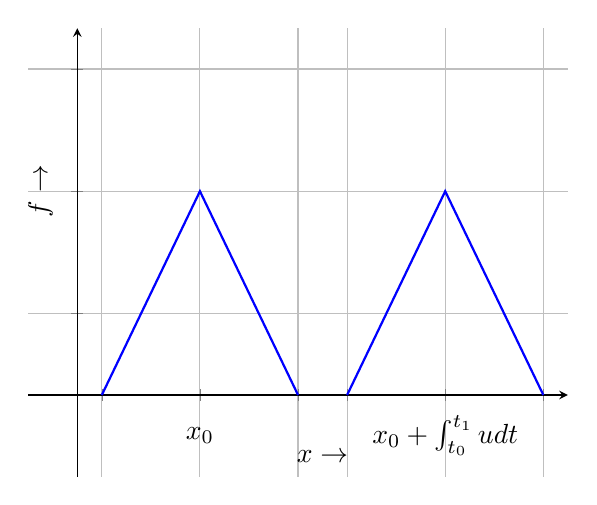
\begin{tikzpicture}
		\begin{axis}[
				% xlabel={$x$},
				% ylabel={$f(x)$},
				axis lines=middle,
				grid=both,
				xmax=10,
				xmin=-1,
				ymax=4.5,
				ymin=-1,
				domain=2:10,
				samples=100,
				xtick={0.5,2.5,4.5, 5.5, 7.5, 9.5},
				ytick={1, 2.5, 4},
				xticklabel=\empty,
				yticklabel=\empty,
			]
			\node at (axis cs:5,-0.75) {$x \rightarrow$};
			\node at (axis cs:-0.75,2.5) [rotate=90] {$f \rightarrow$};
			\draw[thick, blue] (0.5,0) -- (2.5,2.5) -- (4.5,0);
			\draw[thick, blue] (5.5,0) -- (7.5,2.5) -- (9.5,0);
			\node at (axis cs:2.5,-0.5) {$x_0$};
			\node at (axis cs:7.5,-0.5) {$x_0 + \int^{t_1}_{t_0}udt$};
		\end{axis}
	\end{tikzpicture}
	\caption{Triangular property distribution}
	\label{fig:triangularprop}
\end{figure}

\begin{enumerate}[noitemsep]
	\item \textbf{Hyperbolic:} 1$^{st}$ order partial equation $\rightarrow$ 1 family of characteristic equation in real domain.
	\item \textbf{Hyperbolic:} 2$^{nd}$ order partial equation $\rightarrow$ 2 distinct and real set of characteristic equations.
	\item \textbf{Parabolic:} 2$^{nd}$ order partial equation $\rightarrow$ 2 equal and real set of characteristic equations.
	\item \textbf{Elliptical:} 2$^{nd}$ order partial equation $\rightarrow$ 2 distinct and complex set of characteristic equations.
\end{enumerate}

\begin{align*}
	\frac{\partial f}{\partial t} + u \frac{\partial f}{\partial x} = 0 \;
	 & \begin{cases}
		   u = \text{constant} & \Rightarrow \text{linear PDE },     \\
		   u = u(x,t)          & \Rightarrow \text{linear PDE },     \\
		   u = u(x,t,f)        & \Rightarrow \text{quasi-linear PDE}
	   \end{cases}
\end{align*}

\begin{align*}
	a(x,t,f)\frac{\partial f}{\partial t} + b(x,t,f)\frac{\partial f}{\partial x} = 0 \tag{6.5} \label{eq:quasi-linear-ab}
\end{align*}

Above \myeqref{eq:quasi-linear-ab} is quasi-linear PDE, having characteristic equation in real domain $\Rightarrow \frac{dx}{dt} = \frac{b}{a}$

\begin{align*}
	a(x,t,f)\frac{\partial f}{\partial t} + b(x,t,f)\frac{\partial f}{\partial x} = c(x,t,f) \tag{6.6} \label{eq:semi-linear-abc}
\end{align*}

Above \myeqref{eq:semi-linear-abc} is semi-linear PDE, having characteristic equation in real domain.

\clearpage

\section{Lecture 7 22/01/2025}
General quasi-linear 2$^{nd}$ order PDE:
\begin{align*}
	A\frac{\partial^2 f}{\partial x^2} + B\frac{\partial^2 f}{\partial x \partial y} + C\frac{\partial^2 f}{\partial y^2} + D\frac{\partial f}{\partial x} + E\frac{\partial f}{\partial y} + Ff = G \tag{7.1} \label{eq:genral-quasi-linear-pde}
\end{align*}

i.e. $A,B,C$ can be function of $x,y,f,\frac{\partial f}{\partial x}$ and $\frac{\partial f}{\partial y}$.

To find sign of dicriminant $B^2 - 4AC$ tells the classification of equation:
\begin{align*}
	B^2 - 4AC
	\begin{cases}
		> 0, & \text{ Hyperbolic PDE} \\
		= 0, & \text{ Parabolic PDE}  \\
		< 0, & \text{ Elliptical PDE}
	\end{cases}
\end{align*}

This is analogus to general equation of conic-section curves. Which is general by \myeqref{eq:genral-conic-section}
\begin{align*}
	Ay^2 + Bxy + Cx^2 + Dx + Ey + F = 0 \tag{7.2} \label{eq:genral-conic-section}
\end{align*}
\begin{align*}
	B^2 - 4AC
	\begin{cases}
		> 0, & \text{ Hyperbola} \\
		= 0, & \text{ Parabola}  \\
		< 0, & \text{ Ellipse}
	\end{cases}
\end{align*}

\begin{align*}
	df                                       & = \frac{\partial f}{\partial x}dx + \frac{\partial f}{\partial y}dy \tag{7.3} \label{eq:df}                     \\
	d\Big(\frac{\partial f}{\partial x}\Big) & = \frac{\partial^2 f}{\partial x^2}dx + \frac{\partial^2 f}{\partial x \partial y}dy \tag{7.4} \label{eq:dpfpx} \\
	d\Big(\frac{\partial f}{\partial y}\Big) & = \frac{\partial^2 f}{\partial x \partial y}dx + \frac{\partial^2 f}{\partial y^2}dy \tag{7.5} \label{eq:dpfpy}
\end{align*}

Unknown in \myeqref{eq:df}, \myeqref{eq:dpfpx} and \myeqref{eq:dpfpy} are 2$^{nd}$ order derivatives.

From \myeqref{eq:genral-quasi-linear-pde},
\begin{align*}
	A\frac{\partial^2 f}{\partial x^2} + B\frac{\partial^2 f}{\partial x \partial y} + C\frac{\partial^2 f}{\partial y^2} & = - D\frac{\partial f}{\partial x} - E\frac{\partial f}{\partial y} - Ff + G \tag{7.6} \label{eq:genral-quasi-linear-pde-reodered}
\end{align*}

From \myeqref{eq:dpfpx},
\begin{align*}
	\frac{\partial^2 f}{\partial x^2}dx + \frac{\partial^2 f}{\partial x \partial y}dy & = d\Big(\frac{\partial f}{\partial x}\Big) \tag{7.7} \label{eq:dpfpx-reodered}
\end{align*}

From \myeqref{eq:dpfpy},
\begin{align*}
	\frac{\partial^2 f}{\partial x \partial y}dx + \frac{\partial^2 f}{\partial y^2}dy & = d\Big(\frac{\partial f}{\partial y}\Big) \tag{7.8} \label{eq:dpfpy-reordered}
\end{align*}

Matrix representation of \myeqref{eq:genral-quasi-linear-pde-reodered}, \myeqref{eq:dpfpx-reodered} and \myeqref{eq:dpfpy-reordered}:
\begin{align*}
	\underbrace{
		\begin{bmatrix}
			A  & B  & C  \\
			dx & dy & 0  \\
			0  & dx & dy
		\end{bmatrix}
	}_{\text{det(\textbf{A}) = 0}}
	\begin{bmatrix}
		\frac{\partial^2 f}{\partial x^2}          \\
		\frac{\partial^2 f}{\partial x \partial y} \\
		\frac{\partial^2 f}{\partial y^2}
	\end{bmatrix}
	=
	\begin{bmatrix}
		-D\frac{\partial f}{\partial x} - E\frac{\partial f}{\partial y} - Ff + G \\
		d\Big(\frac{\partial f}{\partial x}\Big)                                  \\
		d\Big(\frac{\partial f}{\partial y}\Big)
	\end{bmatrix}.
\end{align*}

Determintant of $(\textbf{A})$ should be equal to zero, i.e.,
\begin{align*}
	\text{det}(\textbf{A})                                    & = 0                                      \\
	A(dy)^2 - B(dxdy) + C(dx)^2                               & = 0                                      \\
	A\Big(\frac{dy}{dx}\Big)^2 - B\Big(\frac{dy}{dx}\Big) + C & = 0 \tag{7.9} \label{eq:matrix-form-pde}
\end{align*}

Solution of above \myeqref{eq:matrix-form-pde} are 2 characteristic equations:
\begin{align*}
	\frac{dy}{dx} & = \frac{B \pm \sqrt{B^2 - 4AC}}{2A}
\end{align*}

\begin{align*}
	\text{if } B^2-4AC > 0 \Rightarrow & \text{2 distinct Real roots}                 \\
	                                   & \text{Family of char. curve}\in \mathbb{R}   \\
	                                   & \text{Hyperbolic PDE}                        \\
	\text{if } B^2-4AC = 0 \Rightarrow & \text{Real and equal roots}                  \\
	                                   & \text{1 Family of char. curve}\in \mathbb{R} \\
	                                   & \text{Parabolic PDE}                         \\
	\text{if } B^2-4AC < 0 \Rightarrow & \text{Imaginary roots}                       \\
	                                   & \text{Family of char. curves}\in \mathbb{C}  \\
	                                   & \text{Elliptic PDE}
\end{align*}

Examples:
\yellownote{
	Incomplete \\
}
\end{document}
